\documentclass{errata}

\hypersetup{
    pdfauthor={王畅、林肃浩},
    pdftitle={中国化学奥林匹克竞赛初赛讲义·勘误表},
    pdfkeywords={}
}

\addbibresource{references.bib}

\title{中国化学奥林匹克竞赛初赛讲义 \\ \bfseries 勘误表}
\author{王畅 \and 林肃浩}
\date{\today}

\begin{document}
    \maketitle
    本文档的最新版本可访问 \url{https://cchobook.github.io/supplementary_materials/errata.pdf} 下载。

    以下页码等信息参照浙江大学出版社 2023 年 6 月出版之《中国化学奥林匹克竞赛初赛讲义》,ISBN 为 978-7-308-23901-1。条目结尾为提供反馈的读者署名,若无署名则为作者自行订正。

    \begin{Errata}
        \item[第 3 页,例题 1.5 结尾]
            \Orig \ce{2CrO4^{2-} + 3S2O4^{2-} -> 4SO3^{2-} + 2Cr(OH)3 + 2HSO3-}
            \Corr \ce{2CrO4^{2-} + 3S2O4^{2-} + 4H2O -> 4SO3^{2-} + 2Cr(OH)3 + 2HSO3-}
            \Thx{匿名}
        \item[第 65 页,习题 4.37 问题之 2 \cite{otten2009complexation}]
            \Orig 但含 \ce{B} 和 \ce{P} 的某个同族元素的键
            \Corr 但含某两个同族元素之间的键
            \Thx{钟天扬(北师大实验中学)}
        \item[第 85 页,例题 6.2 第 3 行]
            \Orig 得到配酸 \cf{C}
            \Corr 得到二元配酸 \cf{C}
        \item[第 91 页,例题 6.14 第 1 行]
            \Orig 亚磷酸(\ce{H3PO2})
            \Corr 次磷酸(\ce{H3PO2})
        \item[第 98 页,习题 6.34 第 2 行]
            \Orig $\omega(\ce{A})$
            \Corr $\omega(\ce{Xe})$
            \Thx{钟天扬(北师大实验中学)}
        \item[第 109 页,倒数第二段第一句话]
            \Orig 最高全充满……\emph{导带}。
            \Corr 最高全充满的一群分子轨道称为\emph{满带},最高有电子填充的一群分子轨道称为\emph{价带},……,价带之后(含价带)未填满或空的能带称为\emph{导带}。
        \item[第 109 页,倒数第一段第一句话]
            \Orig 填满电子的能级……部分重叠
            \Corr 或者填满的价带和导带有部分重叠(如下图),或者价带就是导带(如上图的 \ce{Li})
        \item[第 119 页,例 7.17 第一句话]
            \Orig 镉离子填入所有的八面体空隙
            \Corr 镉离子按层交替地填入一半的八面体空隙
            \Thx{钟天扬(北师大实验中学)}
        \item[第 141 页,例 8.6 第一式]
            \Orig $-\sum_{i=1}^n \frac{nRT}{V_0+n_0 \Delta V} \Delta V$
            \Corr $-\sum_{i=1}^n \frac{nRT}{V_0+i \Delta V} \Delta V$
        \item[第 188 页,例题 10.19] \Orig N/A \Corr 本题两小问应加题号
        \item[第 271 页,习题 11.103] \Orig 合成路线第一行最后一个产物绘制有误 \Corr 应为 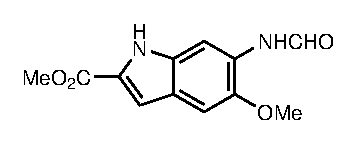
\includegraphics[width=0.3\textwidth]{img/11.103.eps}
        \item[第 331 页,氧族元素问 26] \Orig 连二亚硫酸盐…… \Corr 连二硫酸盐…… \Thx{匿名}
        \item[第 357 页,习题 4.30 答案之 2]
            \Orig \ce{Ni(PEt3)3Cl2} 中 \ce{Ni} 为平面四方结构……填充两个电子。
            \Corr \ce{Ni(PEt3)Cl2} 中 \ce{Ni} 为平面三角形结构,d 轨道分裂为 3 组,其中 $\mathrm d_{xy}, \mathrm d_{yz}$ 简并且能量最低,$d_{z^2}$ 居中,$\mathrm d_{x^2-y^2}, \mathrm d_{xy}$ 简并且能量最高。\ce{Ni} 为 $\mathrm d^8$ 电子构型,除了最高的简并能级各填充一个电子之外,其余轨道都填充两个电子\footnote{注:若按 \ce{Ni(PEt)3Cl2} 处理,则为三角双锥构型,d 轨道分裂为 3 组“211”型式,$\mathrm d_{z^2}$ 能量最高。}。
            \Thx{钟天扬(北师大实验中学)}
        \item[第 369 页,习题 6.25 答案之 3]
            \Orig \ce{2TlO2 + 8HCl -> 2TlCl + 3Cl2 + 4H2O}
            \Corr  \ce{4TlO2 + 4HCl -> 4TlCl + 3O2 + 2H2O}
            \Thx{钟天扬(北师大实验中学)}
        \item[第 369 页,习题 6.26 答案之 2]
            \Orig \ce{SF5}、\ce{F2}、\ce{SF4}、\ce{SF6}
            \Corr \ce{SF5}、\ce{Cl2}、\ce{SF4}、\ce{SF6}
            \Thx{钟天扬(北师大实验中学)}
        \item[第 369 页,习题 6.32 答案之 2]
            \Orig \ce{Hg(NO3)2}
            \Corr \ce{Pb(NO3)2}
            \Thx{钟天扬(北师大实验中学)}
    \end{Errata}

    \renewcommand{\em}{\itshape}
    \renewcommand*{\bibfont}{\footnotesize}
    \renewcommand{\refname}{参考文献}
    \renewcommand{\bibname}{参考文献}
    \printbibliography
\end{document}
